\chapter{\leavevmode\newline The Standard Model of particle physics}
\label{chap:chapter_1}
Several particles were discovered after years of experimental observations, and this led to the development of the Standard Model (SM) during the 1970s. The SM is a Quantum Field Theory (QFT) based on the symmetries of the Lie group, SU(3)$ \times$ SU(2)$ \times$ U(1) \cite{stiller2016full}. It not only describes the fundamental particles and interactions (except for gravitation) but also predicts new particles. The fundamental particles in the SM have a property known as spin and are divided into two main groups: fermions and bosons, as shown in Fig. \ref{fig:sm}.

Fermions obey the Pauli exclusion principle, have $\frac{1}{2}$-spin, and there exists an antiparticle with the same properties but opposite quantum numbers, such as electric charge. They are subdivided into quarks and leptons, with both groups having six particles, and they are further grouped into three generations according to their mass. Quarks are always found in bound states known as hadrons. A meson is formed by a bounded state of a quark and an antiquark, and a baryon is formed by three bounded quarks \cite{stiller2016full, fedi2016studies, grummer2021search}. Quarks have an electrical charge of $+\frac{2}{3}e$ (u, c, t) or $-\frac{1}{3}e$ (d, s, b), as well as a color charge, and can thus interact with the strong force. On the other hand, leptons have an electrical charge of $-1e$ (e, $\mu$, $\tau$) or are neutral (the corresponding neutrinos, $\nu_e, \nu_\mu, \nu_\tau$) and they don't interact with the strong force \cite{bonanomi2021response, bragagnolo2021measurement}.

Bosons have integer spin and are known as force or interaction carriers and are divided into vector and scalar bosons. The Higgs boson is the scalar boson, and it gives mass to the other elementary particles. The vector bosons are related to the fundamental interactions. The photon $\gamma$ is a massless and neutral particle that mediates the electromagnetic interaction between electrically charged particles. The massive bosons, $W^{\pm}$ and $Z$, mediate the weak force between fermions. Finally, gluons mediate the strong interaction between quarks \cite{grummer2021search, bragagnolo2021measurement}.

SM is widely regarded as humanity's most successful theory. It does not, however, explain a number of physical phenomena. For example, the reason why fermions exist in three and only three generations. It does not account for gravity, and to date, there has been no observation of the vector boson responsible for the gravitational interaction, also known as the graviton. It also does not explain why there is more matter than antimatter in the universe, among other properties \cite{grummer2021search, danilov2020measurement}.
\begin{figure}[htp!]
	\centering
	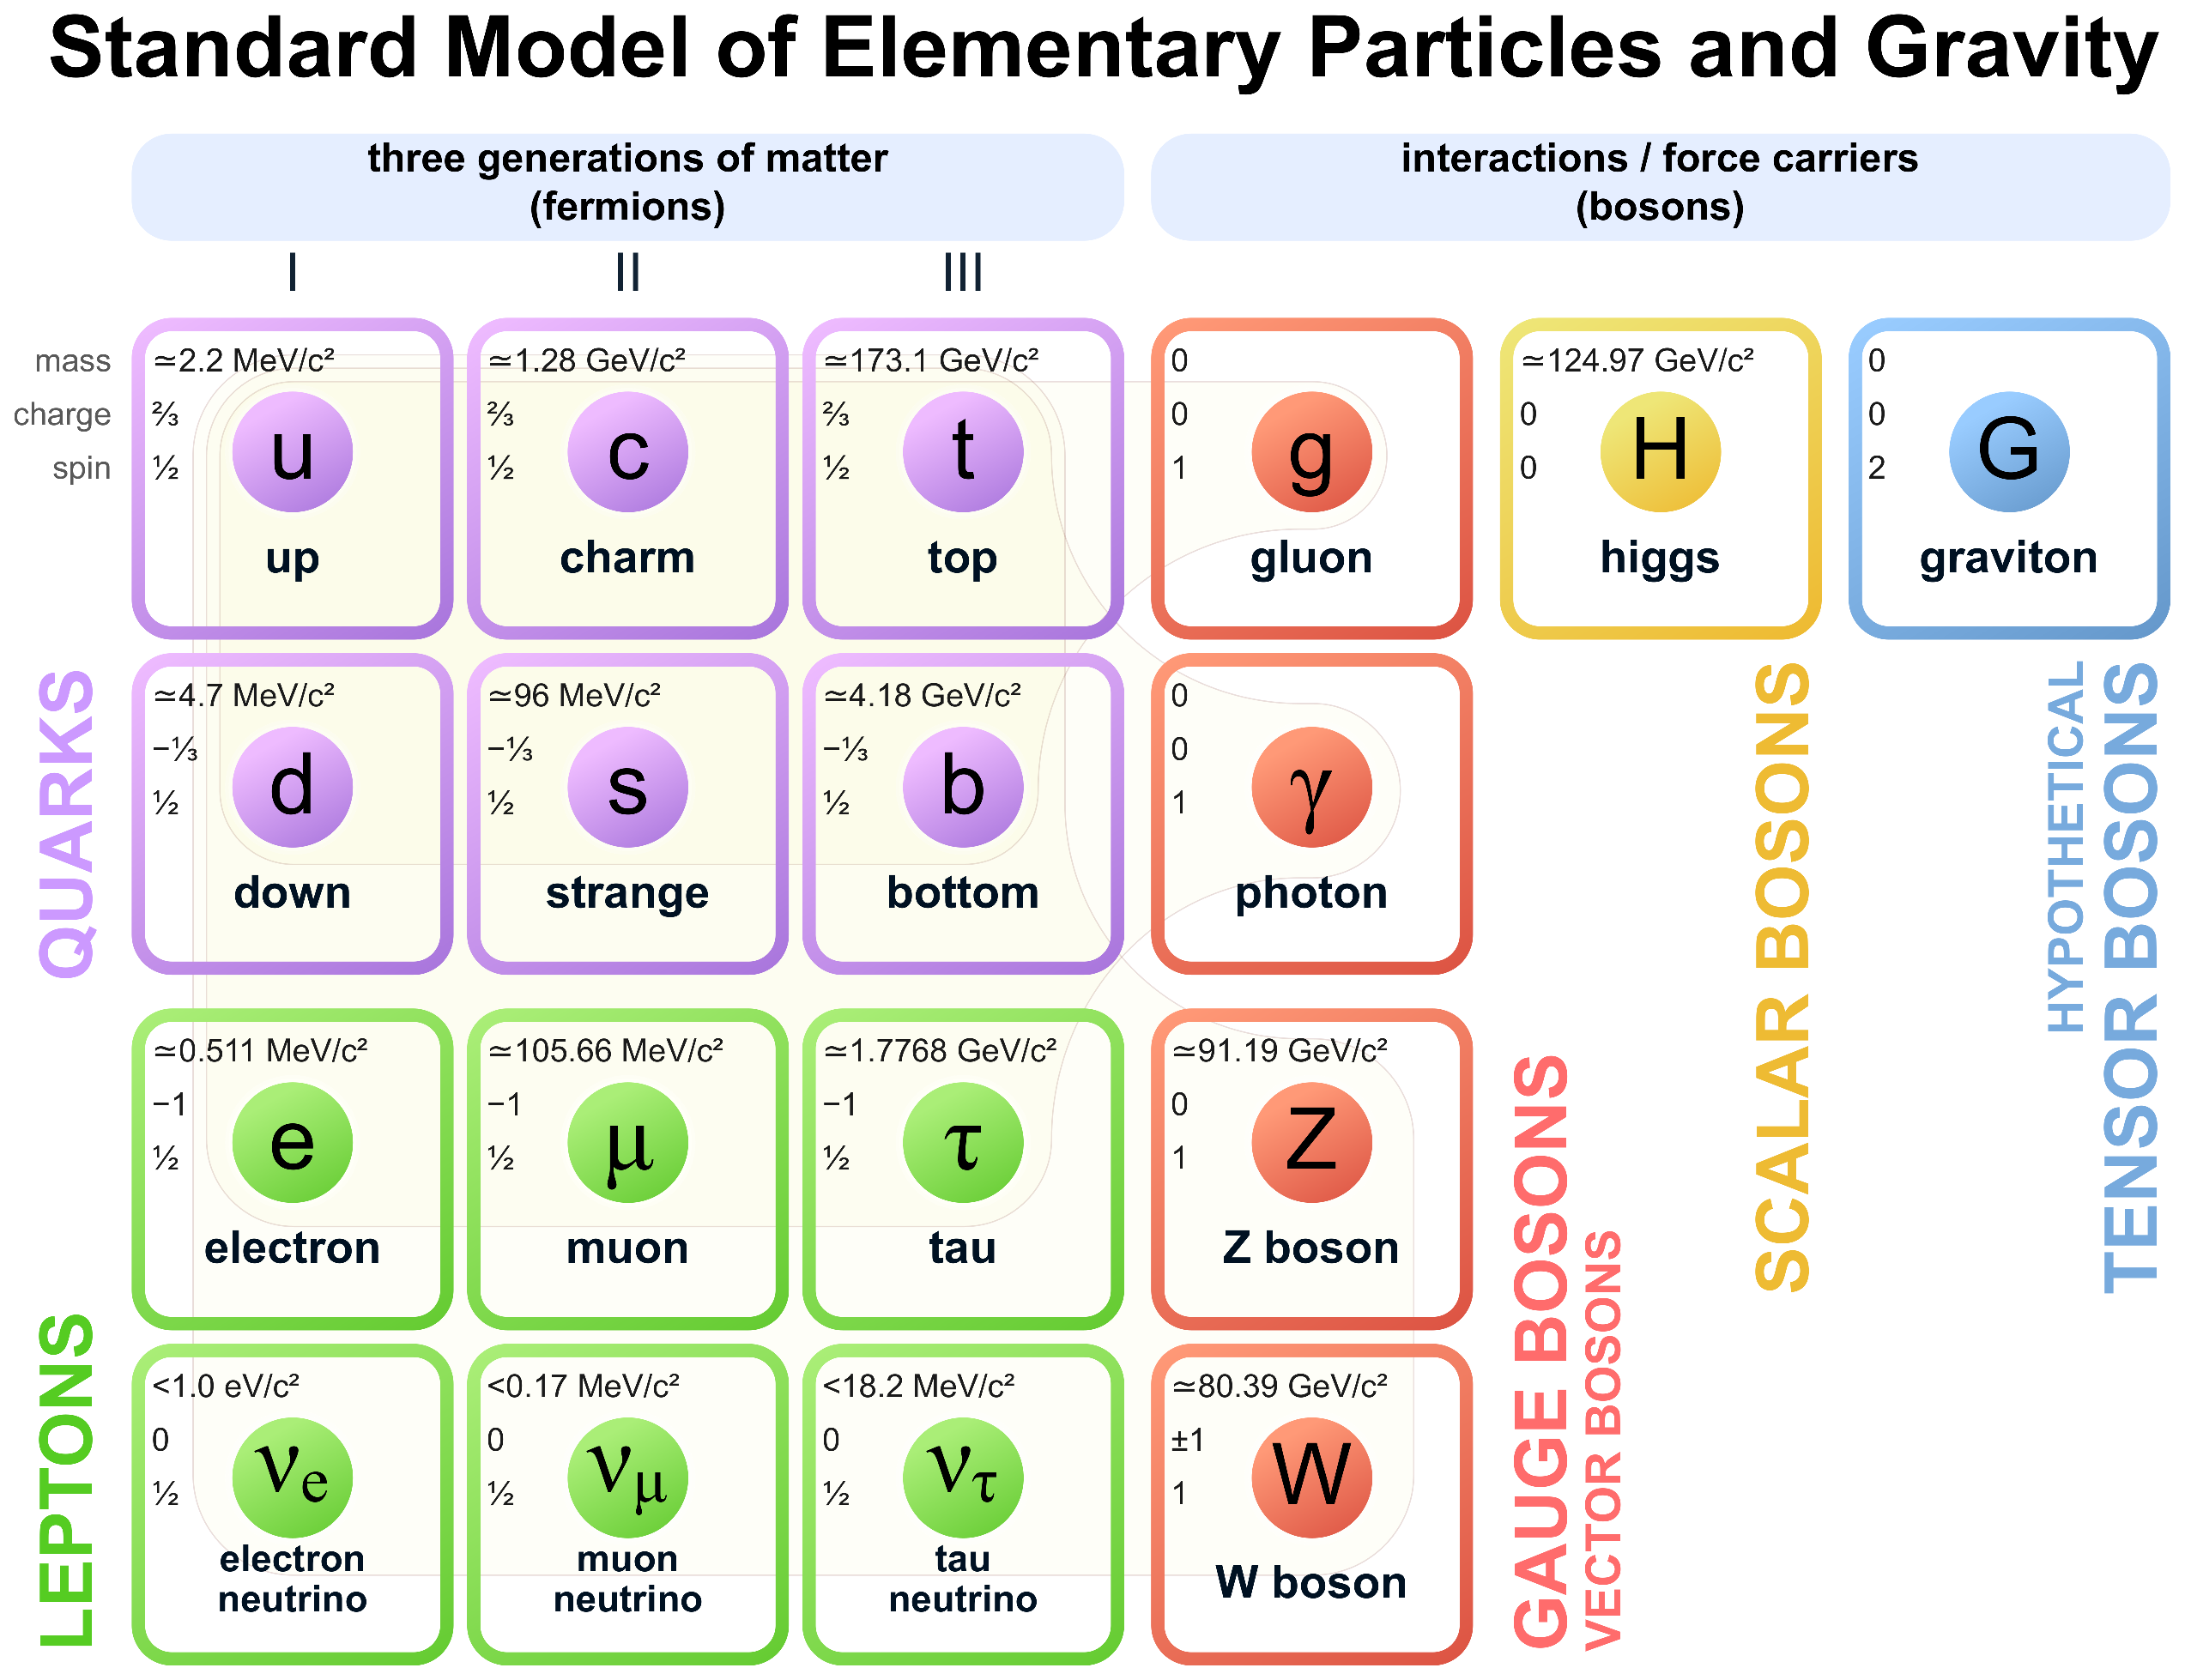
\includegraphics[scale=0.34]{MainContent/Figs/SM.eps}
	\caption{The Standard Model of fundamental particles. Retrieved from \cite{danilov2020measurement}.}
	\label{fig:sm}
\end{figure}

\section{Quantum Chromodynamics}
The theory that describes the strong interactions between colored quarks and gluons is known as Quantum Chromodynamics (QCD). QCD is symmetric under the group SU(3)$_C$, where C stands for color, and similar to the conservation of electrical charge in Quantum Electrodynamics (QED), there is a conserved property known as the color charge with a corresponding anti-color charge. Color charge exists in quarks. This charge comes in three flavors: red (r), blue (b), and green (g). Eight massless gluons mediate the strong interaction and have color charge, allowing them to interact with one another via the strong force \cite{stiller2016full, di2020measurement, thomson2013modern}.

To date, colored quarks have only been observed in colorless bounded states known as hadrons, and not as free particles. This is referred as color confinement, and it is thought to be a direct result of gluons having a color charge \cite{di2020measurement, thomson2013modern}. For a long time, the only hadronic states observed were mesons (one quark and one antiquark) and baryions (three quarks), but in recent years, the LHCb experiment was able to detect  tetraquarks (two quarks and two antiquarks) \cite{aaij2021study} and pentaquarks (four quarks and one antiquark) \cite{aaij2015observation}. The hadronisation process is also a consequence of color confinement.  In this process, a cascade of mesons and baryons known as jets are produced when quarks and gluons group together interactively during gluon-gluon, quark-quark, or quark-gluon collisions \cite{baron2018desarrollo, di2020measurement}.  The HCAL, which is described in the section \ref{cal_sys}, detects jets.

Asymptotic freedom is a property that can also be explained using QCD. When two quarks are brought together, their rate of momentum transfer increases while their coupling constant decreases, this means that their interaction is weaker. If their distance is reduced sufficiently, a point will be reached where quarks and gluons can be considered free particles. This is known as asymptotic freedom, and it is the opposite of color confinement \cite{danilov2020measurement, di2020measurement, sanchez2020search}. 

\subsection{Quark Gluon Plasma}
Extremely high density and energy are required to reach asymptotic freedom, and it is expected that under such conditions, quarks and gluons will de-confine, forming a new state of matter known as Quark Gluon Plasma (QGP) in which they can move freely in the plasma. These conditions were reached shortly after the Big-Bang, therefore, QGP is of high interest in Cosmology \cite{aziz2021z}. Only ultra-relativistic heavy-ion collisions can produce this state. Aside from the LHC experiment, which is described in the following chapter, the BNL's Relativistic Heavy-Ion Collider (RHIC) can produce such collisions \cite{villatorodetection}. 

A phase diagram, as shown in Fig. \ref{fig:qgp}, can be used to summarize the transition mentioned above. Two main regions are depicted in the graphic.  The first region, known as hadron gas, is characterized by low energies and densities, and quarks and gluons are confined into hadrons in such conditions. When a critical point is reached, the transition to the second region, QGP, takes place. QGP is then distinguished by high energies and densities, as well as unbounded quarks and gluons. Direct observations of matter in the QGP state are not possible, their properties can only be inferred by studying the hadrons final states. \cite{villatorodetection, parkkila2021quantifying}.

\begin{figure}[htp!]
	\centering
	\includegraphics[scale=0.34]{MainContent/Figs/QGP.png}
	\caption{Phase transition into the Quark Gluon Plasma (QGP). Retrieved from \cite{parkkila2021quantifying}.}
	\label{fig:qgp}
\end{figure}
\section{$B^0_s$}
\label{sec:b0s}
This thesis focuses on the $B^0_s$ meson, which is made up of of an anti-beauty quark ($\bar{b}$) and a strange quark (s) and its corresponding antiparticle, the $\bar{B^0_s}$, composed of b and $\bar{s}$ \cite{mejia2012medida}. This meson has a mass of $5366.88 \pm 0.14$ MeV and a lifetime of $1.516\pm 0.006 \times 10^{-12}$ s \cite{pdgstrange}. $B^0_s$ mesons undergo a rapid transition into $\bar{B^0_s}$, and vice versa due to the weak interaction. This is referred to as a flavor mixing process, more information can be found in \cite{greevenanalysis, mejia2012medida}. In such transitions, antimatter may decay more often than matter, this is known as charge-parity (CP) violation. The SM, however, does not provide sufficient evidence of CP violation that explains the imbalance of matter and antimatter, as outlined in the previous chapter \cite{greevenanalysis, cern2020lhcb}. $B^0_s$ is an excellent candidate for studying CP violation in depth, as well as some properties of the SM and the physics beyond it.

\subsection{The $B^0_s \to J/\psi \ \phi(1020)$ channel}
\label{subsec:channel}
There are multiple decay channels for the $B^0_s$ meson. However, only the decay into the mesons $J/\psi$ and $\phi(1020)$, denoted as $B^0_s \to J/\psi \ \phi(1020)$, is considered in this manuscript. Aditionally, the decays $J/\psi \to \mu^{+} \mu^{-}$ and $\phi(1020) \to K^{+} K^{-}$ are chosen. The total branching ratio of this decay is:
\begin{equation}
	\label{eq:br}
	\begin{split}
	\mathcal{B} \left(B^0_s \to J/\psi \ \phi(1020) \right) \cdot	\mathcal{B} \left(J/\psi \to \mu^{+} \mu^{-} \right) \cdot \mathcal{B} \left(\phi(1020) \to K^{+} K^{-} \right)  \\
	 = ((1.08 \pm 0.08) \times 10^{-3}) \cdot ((49.2 \pm 0.5) \times 10^{-2}) \cdot ((5.961 \pm 0.033) \times 10^{-2}) \\ = (3.17 \pm 0.24) \times 10^{-5}
	\end{split}
\end{equation}
Although this decay is relatively rare \cite{bragagnolo2021measurement}, it is especially interesting because it allows for a clear observation of CP violation, as well as a precise reconstruction of the $B^0_s$ and the measurement of its mass. The reconstruction process will be explained in detail in Chapter 3.